\section{EEPROM, FLASH a SSD}
\label{sec:eeprom-flash-ssd}
Jedná se o postupné vyvíjení pamětí EEPROM až do pamětí SSD.
Ve všech případech se jedná o paměti non-valitilní a statické, tudíž data zaznamenávají i po odpojení od zdroje el. proudu a data se nemusí obnovovat.
Každou z těchto pamětí je také možné elektricky programovat, tudíž není nutné mazat obsah paměti pomocí UV jako tomu bylo u EPROM.
U těchto pamětí se mění způsob zápisu do paměti i způsob čtení z ní.
Dále má každá paměť rozdílný počet maximálních R/W cyklů, rychlost, přístupovou dobu, cenu, použití a způsob připojení do PC.
\subsection{EEPROM}
\begin{vwcol}[widths={0.6, 0.4}]
  Jedná se o první technologii elektricky programovatelné paměti.
  Zápis a mazání paměti probíhá buňku po buňce.
  Používá transistory MNOS.
  Její počet R/W cyklů je 100 000 cyklů.
  Dnes se používá například pro firmware televizí nebo monitorů.\\
  \vspace*{-1.5cm}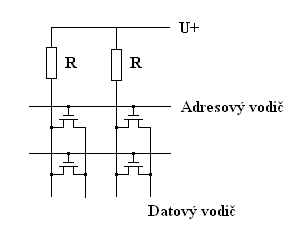
\includegraphics[width=0.3\linewidth]{TVY-POS/EEPROM-FLASH-SSD/EEPROM.png}
\end{vwcol}
\subsection{FLASH}
Zápis a mazání paměti probíhá po blocích.
Tudíž zápis trvá sekundy oproti minutám u EEPROM.
Tato rychlost přichází za cenu menší životnosti.
Její počet R/W cyklů je 10 000 cyklů.
Ovšem díky její vyšší paměťové hustotě je cena nižší jak u EEPROM.
Používá se pro BIOS, SD karty, USB flashdiky
\subsection{SSD}
Využívá NAND FLASH paměti.
Zápis a mazání paměti tudíž také probíhá po blocích.
V dnešní době se používá jako náhrada pevného disku.
Oproti pevnému disku nemá žádné pohyblivé části, tudíž má nižší přístupovou dobu.
Využívá technologie "wear-leveling", která rovnoměrně rozdělenuje zátěž po celém disku.
Má rychlejší rozhraní jak FLASH paměť - SATA, NVME, PCIE.
Umožňuje využití takzvané 3D NAND.
\subsection{Technologie disků}
\subsubsection{3D NAND}
SSD Technologie, která umožňuje zápis více bitů na jednu buňku paměti.
Většinou zařízené pomocí možnosti ukládání více hladit napětí v buňce.
Podle této hladiny lze poté určit správné hodnoty bitů.
Snižuje výdrž disku.
Dělí se na: SLC (Single level cell), MLC (Multi level cell), TLC (Triple level cell) a QLC (4)
\subsubsection{DRAM Cache}
Při výběru SSD disku je vhodné zvolit disk s DRAM Cache, jelikož umožňuje mnohonásobně zvýšit rychlost zápisu a čtení.
\subsubsection{S.M.A.R.T.}
Technologie, která sleduje stav disku.
Dokáže počítači nahlásit všelijaké metriky jako počet zapnutí, počet vadných sektorů a jiné.
Sleduje se pomoci ní životnost disku.
